\begin{figure}[]
\centering
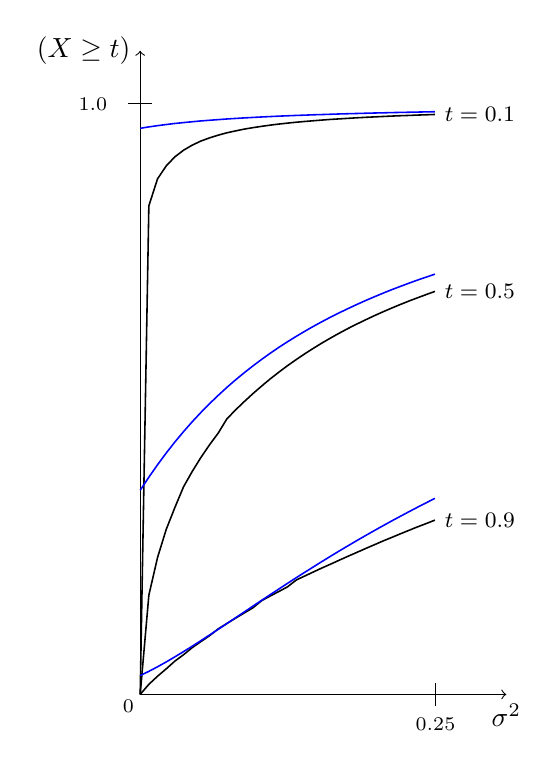
\begin{tikzpicture}[xscale=15, yscale=7.5]%[xscale=10, yscale=5]
\draw[->] (0,0) -- (0.31,0) node[anchor=north] {$\sigma^2$};
\draw[->] (0,0) -- (0,1.09) node[anchor=east] {$\p(X\ge t)$};
\foreach \t in {0.1,0.5,0.9}{
	\draw[domain=0:0.25, color=black, line width=0.20mm, samples=35] 
		plot (\x,{((\x/(\x+\t))^(\x+\t)*(1.0/(1-\t))^(1-\t))^(1.0/(\x+1))}) node [right] {\footnotesize $t=\t$};
	\draw[domain=0:0.25, color=blue, line width=0.20mm, samples=35] 
		plot (\x,{e^(-\t*\t/(4*(1.0/17+\x/2)))}) node [right] {};
}

\draw (0.25,-0.02) -- (0.25,0.02);
\draw (-0.01,1) -- (0.01,1);
\draw	(0.25,-0.05) node{{\scriptsize $0.25$}}
		(-0.01,-0.02) node{{\scriptsize $0$}}
		(-0.04,1) node{{\scriptsize $1.0$}};
\end{tikzpicture}
\caption{The plots of $\p(X\ge t) \le \min_s\E[\exp(sX)]\exp(-st)$ against $\sigma^2$ with $\E[\exp(sX)]$ via equations \ref{eq:part1} (black) and \ref{eq:part3} (blue) with $D=1$, we notice that equation \ref{eq:part3} generally captures the relevant shape and magnitude of the more accurate equation except in region of small $\sigma^2$ where the bound is overly weakened.}
\label{fig:graph2}
\end{figure}